% REVIEW DRAFT (2026-10-18) of the explainer, restructured around the broader question (learning what to change).
% Spoken style for a listener with no background. Every number: records/CORA_SUMMIT_CLAIM_LEDGER_20261017.md.
% The original explainer (docs/summit_poster/explainer.tex) is preserved unchanged.
\documentclass[11pt]{article}
\usepackage[a4paper, margin=2.3cm]{geometry}
\usepackage[scaled]{helvet}
\renewcommand{\familydefault}{\sfdefault}
\usepackage[T1]{fontenc}
\usepackage{microtype}
\usepackage{xcolor}
\usepackage{enumitem}
\usepackage{array}
\usepackage{booktabs}
\usepackage{graphicx}
\usepackage{needspace}
\graphicspath{{../summit_poster/}}
\definecolor{ink2}{HTML}{52514E}
\definecolor{accent}{HTML}{2A78D6}
\pagestyle{plain}
\pdftrailerid{}
\setlength{\parindent}{0pt}
\setlength{\parskip}{0.6em}
\setlist{itemsep=0.25em, topsep=0.2em}
\newcommand{\cue}[1]{{\color{ink2}\textit{[#1]}}\par}
\newcommand{\bigpart}[1]{\par\needspace{10\baselineskip}\vspace{1.2em}{\Large\bfseries #1}\par\vspace{0.1em}}
\newcommand{\panel}[1]{\par\needspace{7\baselineskip}\vspace{0.7em}{\large\bfseries\color{accent}#1}\par\vspace{0.05em}}


\begin{document}
{\LARGE\bfseries Learning what to change: the poster, explained\par}
\vspace{0.3em}
{\raggedright\color{ink2} REVIEW DRAFT, 18 October; for Toni, Chris and Pierce before anything is printed. Read the plain
text aloud. Grey lines in brackets are notes to you. Every number is in
\texttt{records/CORA\_SUMMIT\_CLAIM\_LEDGER\_20261017.md}, with its scope.\par}

\panel{If you only have 20 seconds}
I study how a reasoning system can tell \emph{what to change} when it fails. Is the problem the way it sees
the objects, the rule it applies, or simply not having enough evidence? My system, CORA, solves puzzles by
writing small programs. It can now notice when it has only memorized an answer, build a missing rule, check
the rule on examples it has not seen, and use it. That worked on one practice puzzle and on one real ARC
puzzle. What I have not shown yet is that learning from the failure is what made the difference: a version
that ignores the failure did just as well. That gap is my research question.

\bigpart{Part 1. The question}

\panel{1. The problem}
\cue{column 1, top}
People can learn a new kind of reasoning from a handful of examples, even when the meaning of the
examples is new. For a machine this breaks into three questions:
\begin{enumerate}
  \item \textbf{Representation.} Can it find the right things to reason about (objects, parts, relations) in
    data it has not seen before?
  \item \textbf{Rules.} Can it discover the executable rules that act on those things?
  \item \textbf{Revision and transfer.} When it fails, can it tell which of these was wrong and fix the right
    one? And does that skill of fixing carry over to a domain with completely different meaning, for
    example from visual puzzles to molecular measurements?
\end{enumerate}
These questions were shaped in discussion with Toni Kazic.

\panel{2. Why one solved puzzle proves little}
Many different programs can reproduce every example and still disagree on a new case. On 60 practice puzzles,
CORA's object reasoner often found programs that matched every example perfectly and were wrong on the test.
That happened in 26 puzzles (27 without its saved library). It had memorized the examples instead of
finding the rule.

A failure can come from three places, and each needs a different fix:
\begin{itemize}
  \item the \textbf{representation}: the objects were cut up wrongly;
  \item the \textbf{rule}: the right operation was missing;
  \item the \textbf{evidence}: the examples do not decide between several rules.
\end{itemize}
Choosing the wrong fix can break things that used to work.

\bigpart{Part 2. Why ARC is a good place to study this}

\panel{3. The puzzles}
\cue{any grid on the poster}
Each ARC puzzle gives two to five example pairs of coloured grids and one new input. The solver must
produce the exact output. There is no partial credit and no training on the answer. That makes ARC a
controlled laboratory:
\begin{itemize}
  \item the evidence is sparse;
  \item every answer can be checked exactly;
  \item many puzzles need a transformation that no fixed list of operations covers.
\end{itemize}
It is not the end goal. It is the place to test the reasoning procedure before trying it in science, where
checking is much harder.

\bigpart{Part 3. What CORA actually demonstrates}

\panel{4. Four achievements, four different statuses}
\cue{the table in column 1}
\begin{center}
\begin{tabular}{@{}p{0.55\linewidth}p{0.36\linewidth}@{}}
\toprule
achievement & status today \\ \midrule
detect certain reasoning failures & built, with limits \\
construct and verify an executable correction & shown on one synthetic and one exposed real puzzle \\
learn to choose better revisions from failures & \textbf{not established} \\
transfer a revision policy to biology & \textbf{not tested} \\ \bottomrule
\end{tabular}
\end{center}
Keeping these four apart is what makes the larger idea credible.

\needspace{26\baselineskip}\panel{5. Where CORA fails on real puzzles}
\cue{the bar chart in column 2}
\begin{center}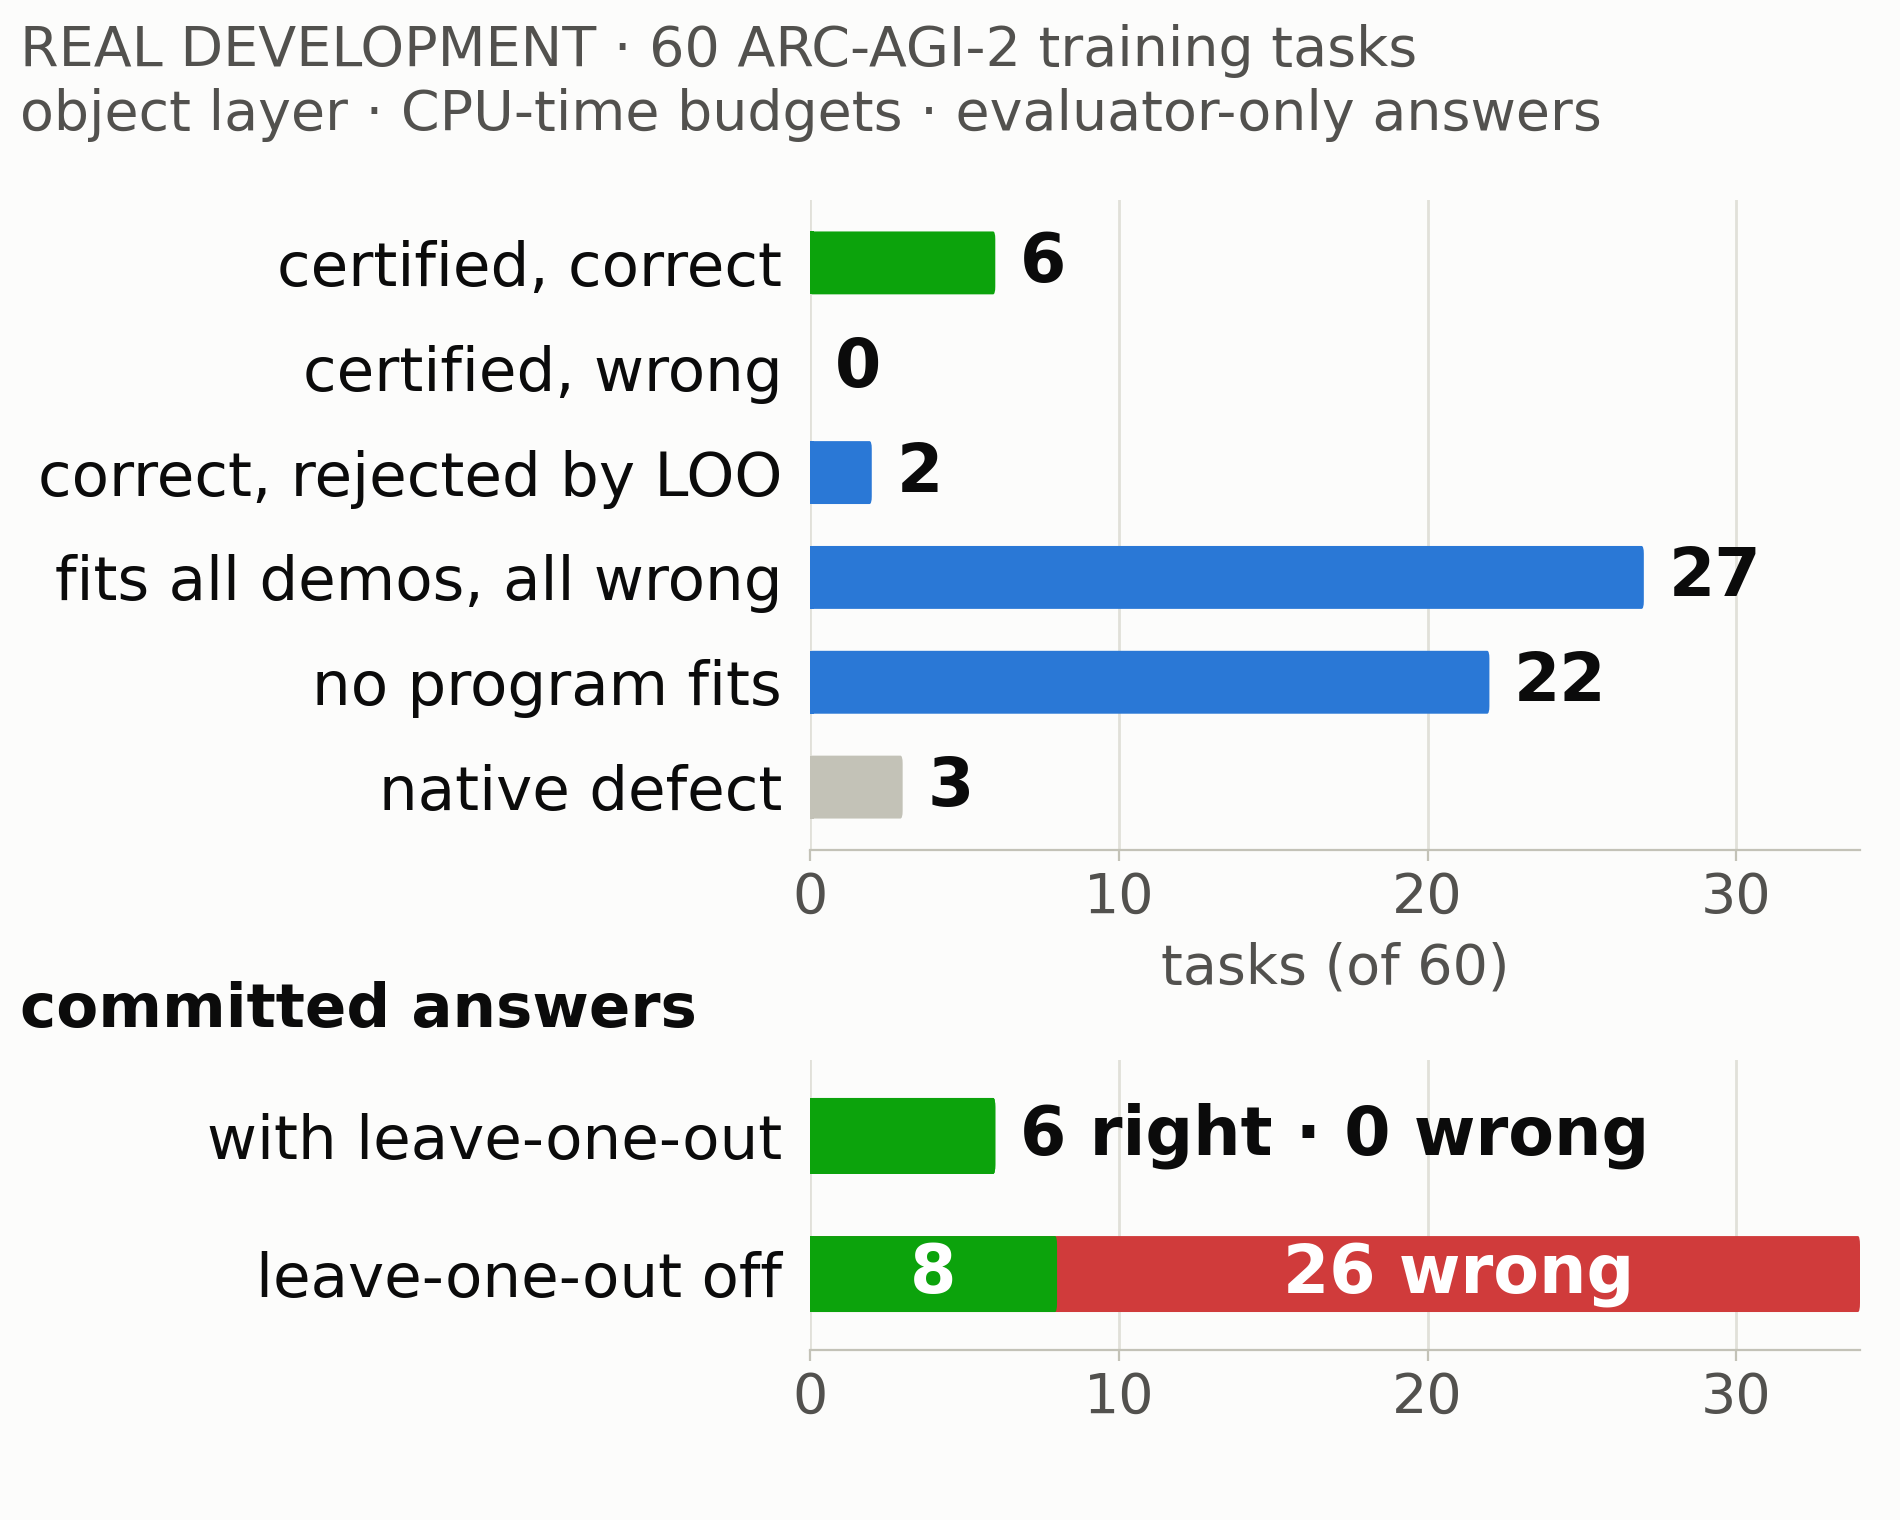
\includegraphics[width=0.82\linewidth]{figures/fig_failure_funnel_dev60.png}\end{center}
I measured, step by step, where CORA's object reasoner fails on 60 real practice puzzles.
\begin{itemize}
  \item Its own check is careful: it accepted 6 answers, and all 6 were right.
  \item The big problem is memorizing. In 26 puzzles (27 without the saved library, as in the chart) every
    program that fitted the examples was wrong.
  \item A correct candidate existed on 8 puzzles. With the check switched off it would have answered 8 right
    and 25 wrong (26 in the chart's configuration).
  \item Giving it three times the search time fixed none of the memorized puzzles.
\end{itemize}

\needspace{26\baselineskip}\panel{6. Building a missing rule: the practice puzzle}
\cue{the small figure, if shown}
\begin{center}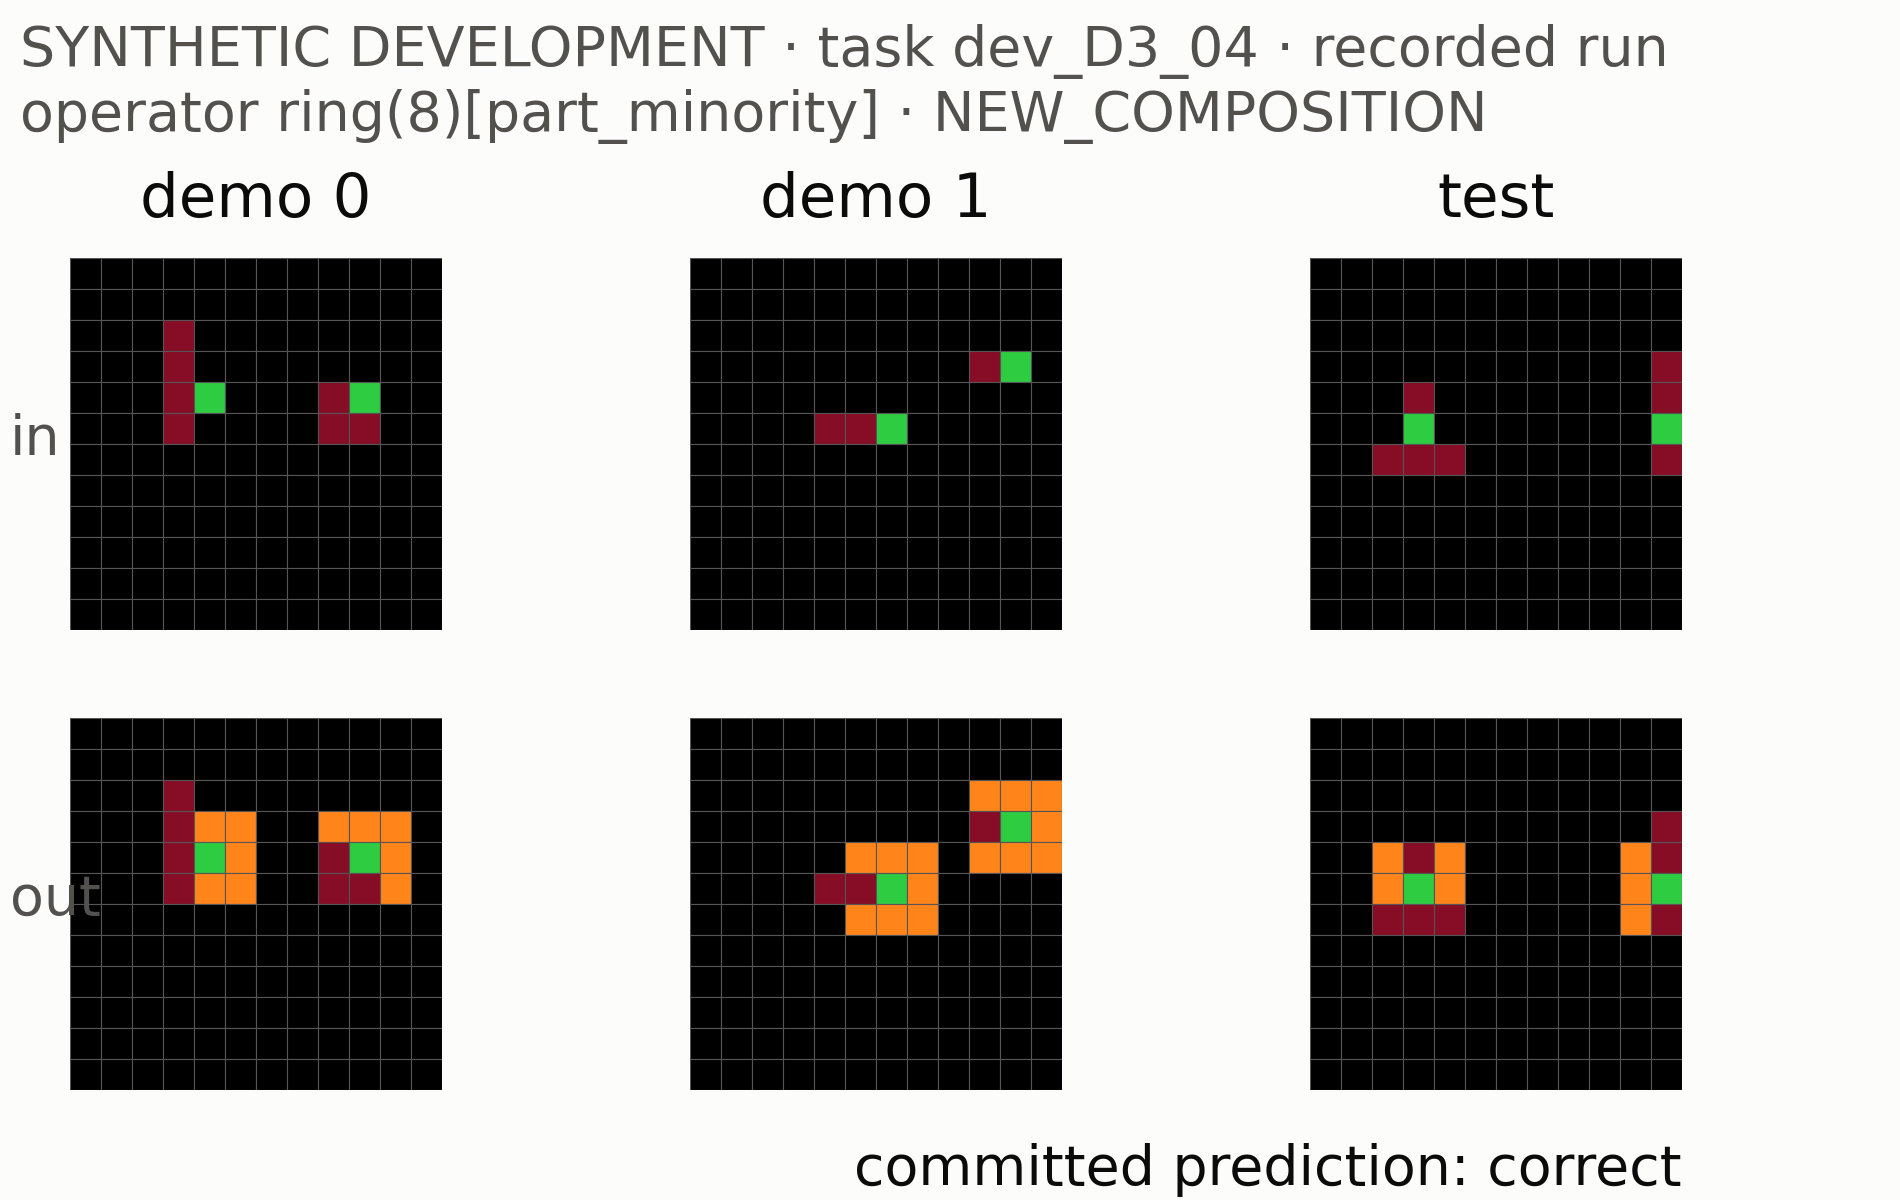
\includegraphics[width=0.82\linewidth]{figures/fig_fhr_witness_dev_D3_04.png}\end{center}
When the solver could only memorize, CORA looked at exactly which objects it had memorized. From a fixed
list of building blocks (37,750 possible rules) it built one: a ring around the odd-coloured cell. It
plugged that rule into the unchanged solver and tested it three times, each time hiding one example,
rebuilding the rule from the others and predicting the hidden one. All three passed, and the final answer
was right. Removing the rule broke it again.

The rule is a single step, not a complex one. A version that ignored the failure record found the same rule.

\needspace{26\baselineskip}\panel{7. A real puzzle solved by a built rule}
\cue{the grid figure in column 2; demo: \texttt{run\_demo.sh --real}}
\begin{center}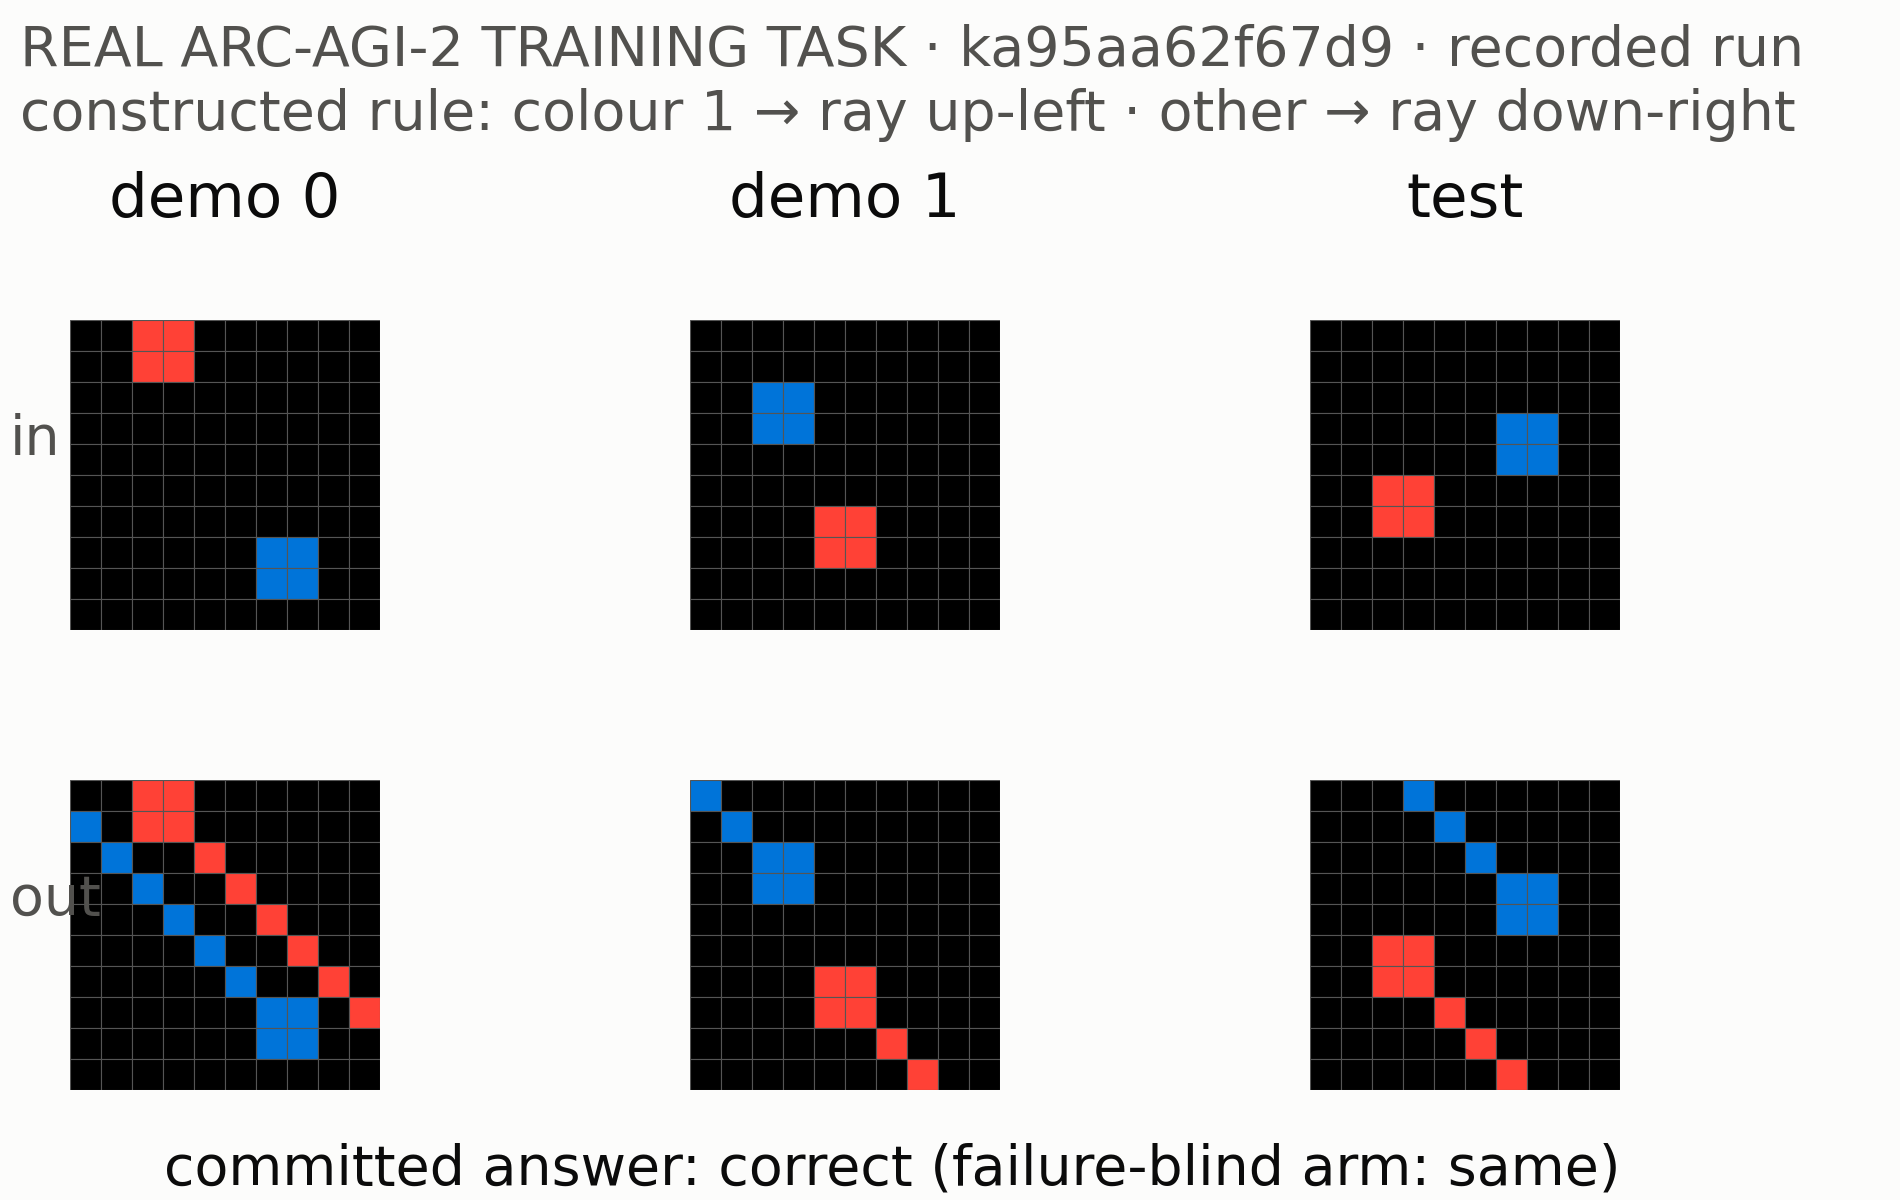
\includegraphics[width=0.82\linewidth]{figures/fig_fhr_real_witness_ka95aa62f67d9.png}\end{center}
This is a real ARC training puzzle. CORA's solver fails it, even with extra search time. My failure analysis
found that each object's change could be described, but not all of them by one rule. So I let a rule say
\emph{where} it applies as well as \emph{what} it does. CORA built: ``blue objects (colour 1) shoot a ray to
the upper left; the others shoot one to the lower right''. It passed all three hidden-example checks, the
solver used it, the solver was restored afterwards, and the answer was right.

The limits:
\begin{itemize}
  \item I found this puzzle through my own analysis;
  \item it is a training puzzle, so it is not a test of generalization;
  \item a version that ignores the failure record found the same rule, from the same evidence;
  \item it was built after my Kaggle entry, so it is not part of that entry.
\end{itemize}

\panel{8. Does learning from the failure actually help?}
\cue{the red ``not established'' block}
This is the central question, and the honest answer today is: not shown.
\begin{itemize}
  \item On the practice puzzles, a constructor that saw the same information but not the failure record
    matched every certified answer.
  \item A pilot on puzzles where the solver understood some objects but not others failed its pre-set
    criterion.
  \item In a frozen 10-puzzle test of the new where-and-what rules, learning from the failure got 2 right and
    the failure-blind version got 1 right. The blind version abstained once, because 15 equally simple rules
    disagreed. One puzzle of difference is not evidence (a sign test gives $p = 0.5$).
  \item I wrote a simple rule book that chooses which kind of fix to try from the solver's trace. Tested on
    recorded runs, it missed the one puzzle that extra search time had fixed: 6 right against 7.
\end{itemize}
So \textbf{building a rule} and \textbf{learning which revision to make} are different capabilities. Only the
first is demonstrated.

\panel{9. Why construction rarely fires}
In the Kaggle practice run, the construction step could apply to 62 puzzles:
\begin{itemize}
  \item 20 left no trace of memorizing;
  \item 39 left traces that no rule fitted;
  \item 2 ran out of time;
  \item 1 rule fell apart in its checks.
\end{itemize}
Looking closely at 25 real cases, 18 needed operations the building-block list simply does not contain.
That is a limit of the language I gave it, not of search. Learning the language itself is the larger problem,
which my separate Step B experiment studies.

\panel{10. What is designed by hand, and what is automatic}
\begin{itemize}
  \item \textbf{Designed by me:} the trigger (``objects the solver could only memorize''), the list of
    building blocks, and the checks.
  \item \textbf{Automatic:} the choice of rule, the choice of where it applies, and its rebuilding in every
    check.
  \item Hiding one of three examples at a time is a consistency check, not a proof that the rule holds
    everywhere.
\end{itemize}

\bigpart{Part 4. What others already do}

\panel{11. Close relatives}
\cue{``Where this sits'', column 1}
\begin{itemize}
  \item \textbf{Popper} (Cropper and Morel) learns programs by learning from failed hypotheses.
  \item \textbf{DreamCoder} (Ellis and colleagues) and \textbf{LILO} (Grand and colleagues) grow libraries of
    reusable program pieces.
  \item \textbf{Model Discovery Agent} (Kevin Murphy) uses a model's failures to revise hypotheses and design
    experiments. It is the closest idea to the broader question here.
  \item Large neural reasoners and scientific agents are strong and improving fast. They can use tools and
    check their own work, and I do not claim otherwise.
\end{itemize}
What I add is narrower and testable: measuring whether a system chooses \emph{which component} to revise
better than an equally equipped system that does not use the diagnosis. Measuring the damage done by wrong
revisions, and the cost, is part of the test.

\bigpart{Part 5. The experiment that would answer the larger question}

\panel{12. The next test, already running}
\cue{column 3, ``The next falsifiable test''}
On 58 practice puzzles, chosen by a fixed rule before anything ran, I compare:
\begin{itemize}
  \item the solver alone, and with extra search;
  \item learning from the failure;
  \item an equally equipped version that ignores the failure;
  \item a version given someone else's failure record;
  \item a new version that learns \emph{what} to change from what the solver could only memorize, and
    \emph{where} it applies from the contrast with what the solver already explains.
\end{itemize}
The comparisons are decided in advance, with corrections for testing several things at once. I will report
the result only after it is checked, whatever it is.

\panel{13. From puzzles to science (proposed, not tested)}
\cue{column 3, ``Scientific prediction''}
The same question matters in biology. When a model of molecular measurements fails, should it change how
it represents the measurements, revise its hypothesis, or ask for a new experiment?

What might transfer is the \emph{revision policy} and the checking discipline, not any puzzle operation.
I separate four levels:
\begin{enumerate}
  \item the same software runs in both domains;
  \item the same method trained separately in each;
  \item a policy learned on ARC, frozen, improves revision decisions on the biological task;
  \item those decisions improve independently validated predictions.
\end{enumerate}
Only the fourth would be a biological result, and none of them has been tested.

A biological check also differs from an ARC check: it needs a tolerance, real replicates, held-out
conditions and, in the end, an experiment. The concrete problem is being defined with Pierce and Toni;
nothing here uses their data.

\bigpart{Part 6. Benchmark context}
\begin{itemize}
  \item Official Kaggle ARC-AGI-2 public score of my own solver, native CORA: \textbf{0.00}.
  \item A careful reproduction of a published neural method (NVARC, Qwen3-4B): \textbf{27.64}. It is not my
    invention and not CORA.
  \item On 18 October I submitted a research entry that runs CORA's construction step. It scored
    \textbf{0.00}, as expected: in its practice run it added no answers, and the where-and-what rule above was built after it.
\end{itemize}

\bigpart{Part 7. How to reproduce what you see}
{\raggedright
\begin{itemize}
  \item \textbf{Review poster and this explainer:}
    \texttt{docs/summit\_20261023\_reframe/poster\_review.tex} and \texttt{explainer\_review.tex}, built with
    pdflatex. The figures are in \texttt{docs/summit\_poster/figures/}, drawn from hash-pinned records
    (\texttt{scripts/summit\_figures.py}; hashes in \texttt{figures/PROVENANCE.json}).
  \item \textbf{Both demos} (offline replays, numpy only; each refuses to run if a recorded file's hash
    differs): \texttt{sh docs/summit\_demo\_20261023/run\_demo.sh} (practice puzzle) and
    \texttt{run\_demo.sh --real} (the real puzzle).
  \item \textbf{The experiments:} the failure analysis is \texttt{records/CORA\_REVISION\_ROOT\_CAUSE\_20261018.md};
    the frozen 10-puzzle test is \texttt{records/CORA\_FHR\_GUARD\_PROBE\_PROTOCOL\_20261018.md}; the
    running 58-puzzle test is \texttt{records/CORA\_FHR\_GUARD\_GENERALIZATION\_PROTOCOL\_20261018.md}.
\end{itemize}\par}
\end{document}
